\label{app:chap5}

\section{Position acquisition from pixel to world coordinates}

\begin{figure}[H]
    \centering
    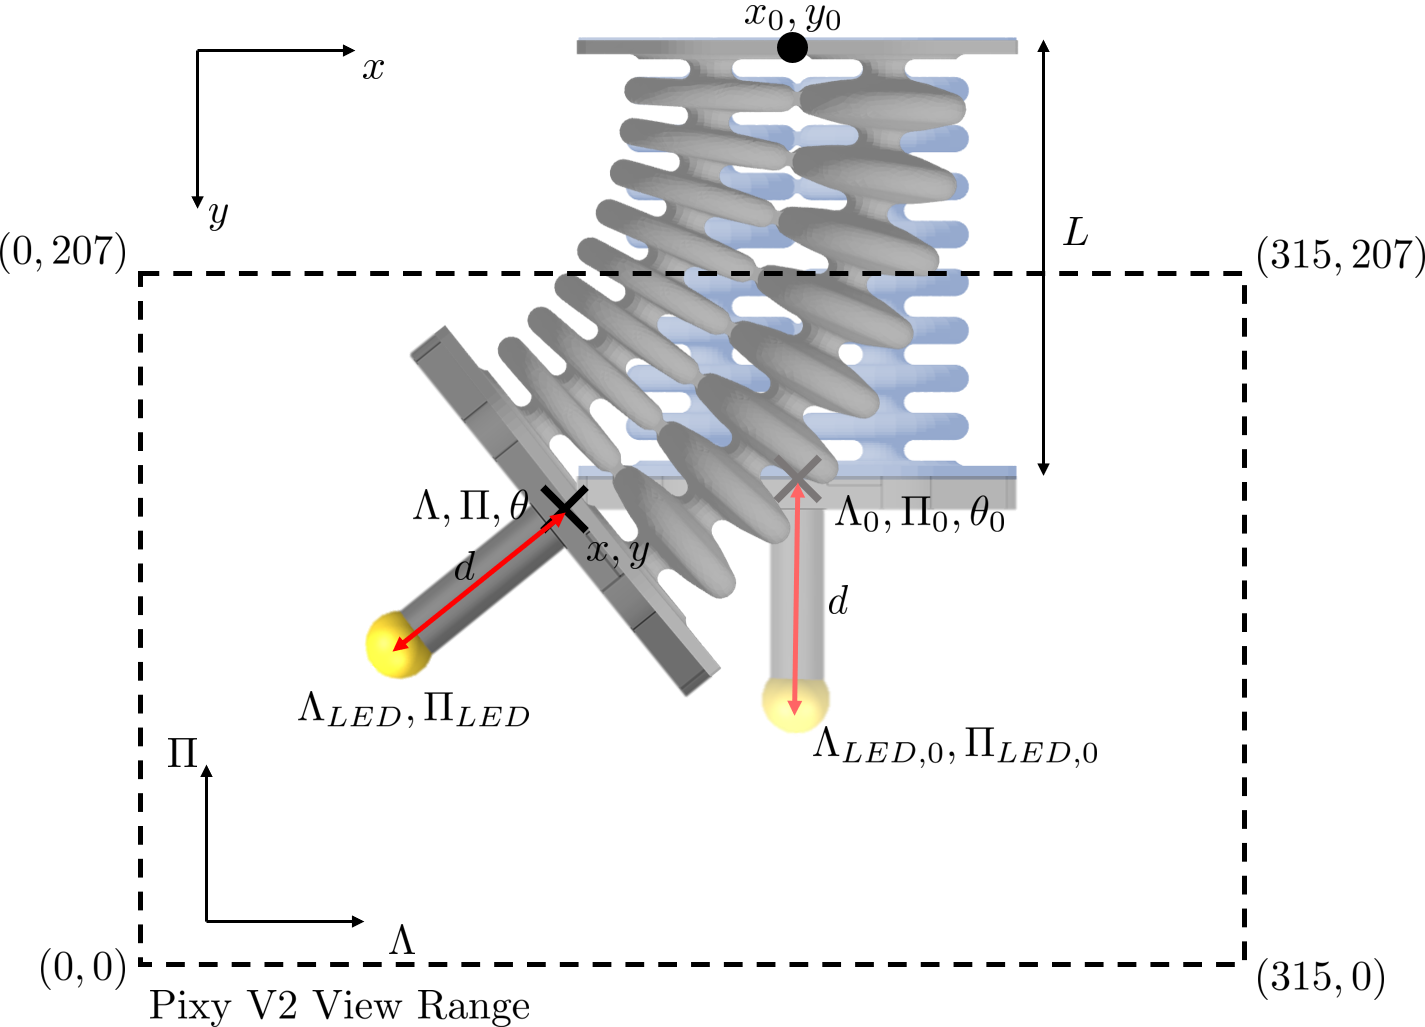
\includegraphics[width = 0.95\textwidth]{Figures/Appendix5/pix2w.png}
    \caption{Vision system coordinate frame.}
    \label{figapp5:px2w}
\end{figure}


Figure \ref{figapp5:px2w} displays the vision system coordinate frame, where the dotted lines mark the pixel window. The resolution of the vision system is 207$\times$315, as indicated by the corner coordinates. The pixel values of the end-effector are denoted by $(\Lambda,\Pi)$. The position of the $LED$ marker in pixel coordinates are given by $(\Lambda_{LED},\Pi_{LED})$. Consider the origin of the soft robot in world frame coordinates given by $(x_0,y_0)$. Note that this position can be outside of the vision system's viewing range. The initial end-effector position in pixel coordinates is given by,


\begin{equation}
    \Lambda_0 = \Lambda_{LED,0} + \frac{d}{px2w} \sin(\theta_0) \hspace{20pt} \text{and} \hspace{20pt} \Pi_0 = \Pi_{LED,0} + \frac{d}{px2w} \cos(\theta_0),
\end{equation}

where $d$ is the offset between the LED marker and the end-effector, $px2w$ a constant mapping pixel coordinates to world coordinates. The initial angle is given by $\theta_0$. Likewise, the actual position of the end-effector during operation is given by,


\begin{equation}
    \Lambda = \Lambda_{LED} + \frac{d}{px2w} \sin(\theta) \hspace{20pt} \text{and}    \Pi = \Pi_{LED} + \frac{d}{px2w} \cos(\theta).
\end{equation}

Based on the difference between actual and initial position in pixel coordinates, the position in world coordinates can be obtained by, 

\begin{equation}
    x = (\Lambda-\Lambda_0)px2w \hspace{20pt} \text{and} y = L - (\Pi - \Pi_0)px2w. 
\end{equation}










\section{Ellipsoid reference tracking in simulation for relative fast trajectories}


\begin{figure}[H] 
    \begin{minipage}[b]{0.49\linewidth}
     \centering
    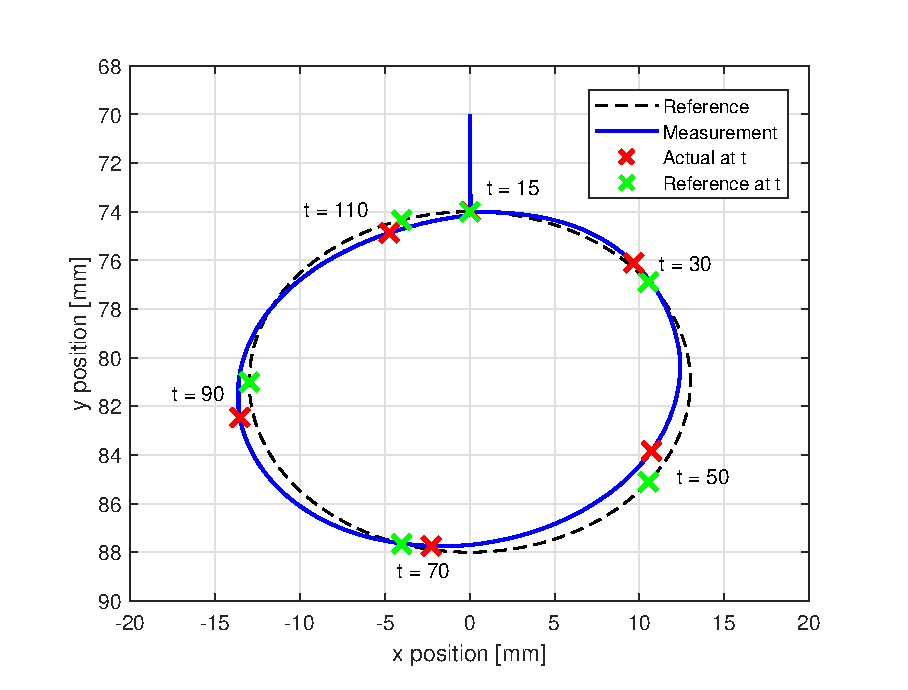
\includegraphics[width=\linewidth]{Figures/Chapter5/ellipsxy.eps} 
    \caption{Position in the x,y-plane for the ellipsoid reference path. } 
    \label{app5:xysim} 
       \end{minipage} 
    \begin{minipage}[b]{0.49\linewidth}
     \centering
    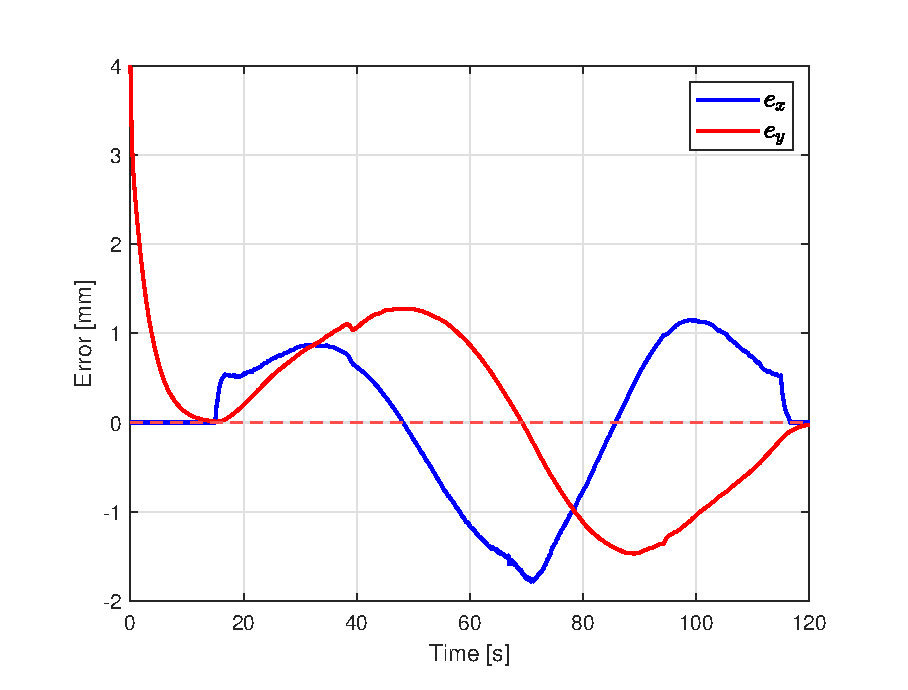
\includegraphics[width=\linewidth]{Figures/Chapter5/errorellips.eps} 
    \caption{Error in the x and y-direction as a function of time for an ellipsoid reference path.} 
    \label{app5:errorxyellipssim} 
    \end{minipage} 
\end{figure}

\begin{figure}[H]
    \centering
    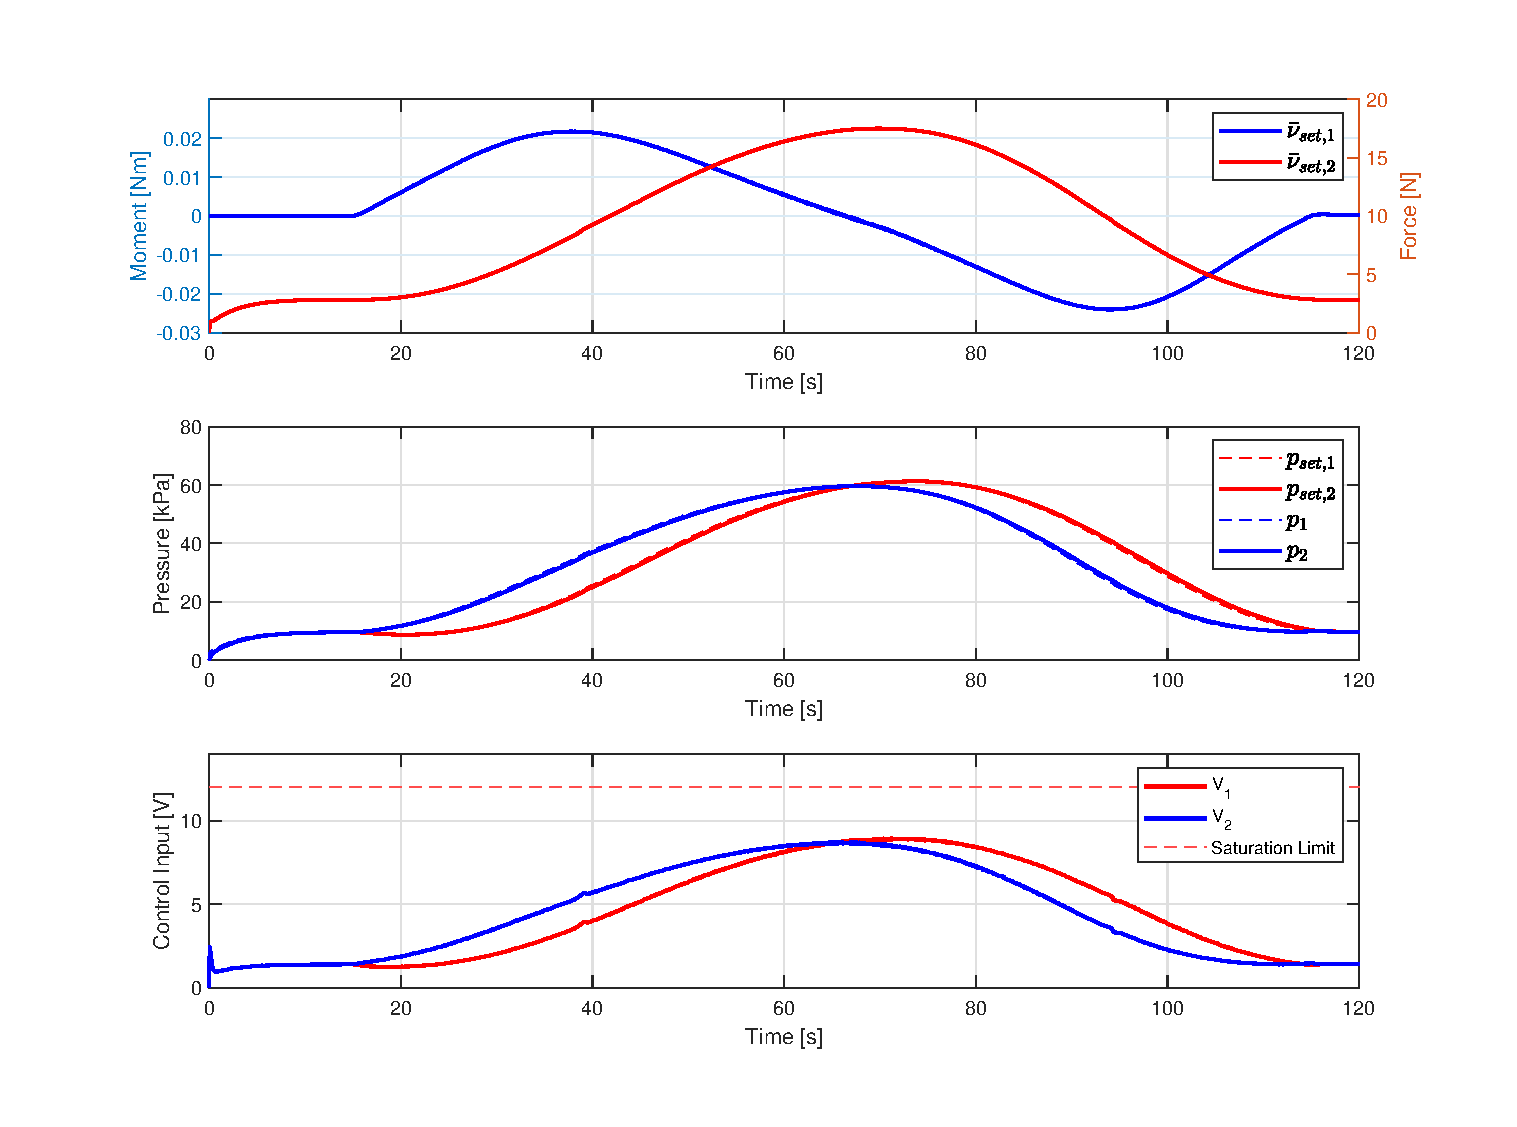
\includegraphics[width = \textwidth]{Figures/Chapter5/inputellipssim.eps}
    \caption{\textbf{Top:} Control signal of model-based controller. \textbf{Middle:} Reference pressure and actual pressure. \textbf{Bottom:} Control input to the air pumps.}
    \label{app5:controlinputellipssim}
\end{figure}
